\documentclass[12pt]{book}
\usepackage[utf8]{inputenc}
\usepackage[german]{babel}	% hyphenation and content headings  %%LOCALIZE

\usepackage[T1]{fontenc}		% Allow Swedish, German etc. letters
\DeclareTextCommand{\nobreakspace}{T1}{\leavevmode\nobreak\ }


\usepackage{titling}
\usepackage[left=2cm, right=2cm,bottom=3cm,top=2cm, paperwidth=297mm, paperheight=210mm, twoside=false]{geometry}

\usepackage[scaled]{helvet}
%\usepackage{tgheros} %alternative to helvet
\renewcommand{\familydefault}{\sfdefault}
\usepackage{sectsty}
\allsectionsfont{\sffamily}
\usepackage[scaled=1.02]{inconsolata}
%\usepackage[scaled]{beramono} %alternative to inconsolata

\usepackage{url}
\usepackage[hidelinks]{hyperref}
\usepackage{wrapfig}
\usepackage{titlepic, graphicx}
\usepackage[usenames,dvipsnames]{xcolor}
\usepackage{array} %to center table cells
\usepackage{parskip} %to have noindent and space between paras
\usepackage{tikz}

\usepackage{titlesec}
\titleformat{\chapter}[hang]{\bf\fontsize{40}{40}\selectfont\centering\vskip-13mm}{}{0pt}{\bf\fontsize{40}{40}\selectfont}
\titleformat{\section}[hang]{\bf\fontsize{24}{24}\selectfont}{}{0pt}{\bf\fontsize{24}{24}\selectfont}
\titlespacing\chapter{0pt}{20pt plus 10pt minus 10pt}{20pt plus 10pt minus 10pt}
\titlespacing\section{0pt}{10pt plus 4pt minus 2pt}{0pt plus 4pt minus 2pt}
\addto\captionsgerman{%%%LOCALIZE
  \renewcommand{\contentsname}%
    {Inhalt}%
}
\usepackage{multicol}

\usepackage{listings}
\lstset{literate=%
%swedish and german letters
{Å}{{\AA}}1
{Ä}{{\"A}}1
{Ö}{{\"O}}1
{Ü}{{\"U}}1
{ß}{{\ss}}1
{ü}{{\"u}}1
{å}{{\aa}}1
{ä}{{\"a}}1
{ö}{{\"o}}1
%danish letters
{æ}{{\ae}}1
{ø}{{\o}}1
{Æ}{{\AE}}1
{Ø}{{\O}}1
}            
% "define" Scala
\lstdefinelanguage{scala}{
  morekeywords={abstract,case,catch,class,def,%
    do,else,extends,false,final,finally,%
    for,forSome,if,implicit,import,lazy,match,%
    new,null,object,override,package,%
    private,protected,return,sealed,%
    super,this,throw,trait,true,try,%
    type,val,var,while,with,yield},
  otherkeywords={=>,<-,<\%,<:,>:,@},
  sensitive=true,
  morecomment=[l]{//},
  morecomment=[n]{/*}{*/},
  morestring=[b]",
  morestring=[b]',
  morestring=[b]"""
}
\usepackage{color}
\definecolor{dkgreen}{rgb}{0,0.6,0}
\definecolor{gray}{rgb}{0.5,0.5,0.5}
\definecolor{dkgray}{rgb}{0.3,0.3,0.3}
\definecolor{mauve}{rgb}{0.58,0,0.82}
 
% Default settings for code listings
\lstset{frame=none, 
  language=scala,
  aboveskip=3mm,
  belowskip=3mm,
  %framesep=2cm,xleftmargin=-10pt,xrightmargin=10pt,
  showstringspaces=false,
  columns=flexible,%flexible ,%fixed
  basicstyle={\ttfamily\selectfont},
  keywordstyle=\bf\ttfamily\selectfont\color{blue},
  commentstyle=\color{dkgreen},
  stringstyle=\color{mauve},
  breaklines=false,
  breakatwhitespace=false,
  tabsize=2,
  numbers=none,stepnumber=1, numbersep=8pt, numberstyle=\small\color{gray}
}

\title{\fontsize{40}{40}\bf\sffamily\selectfont Aufgaben mit Kojo} %%%LOCALIZE
\author{Editor: Björn Regnell \\ \bf www.lth.se/code} %%%LOCALIZE
\titlepic{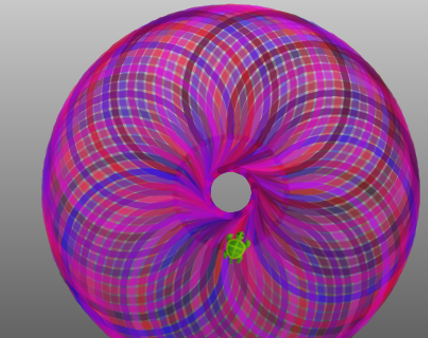
\includegraphics[height=8cm]{../img/cover}}
\date{}
\renewcommand{\thechapter}{} % removes chapter numbers also in table of contents

\begin{document}
\maketitle
\newpage
\thispagestyle{empty}

{ \vspace{250mm}\fontsize{11}{11}\flushleft\selectfont 
\vspace*{\fill}

\begin{center}
\Huge {\bf Aufgaben mit Kojo}\\
\Large {\bf Version}: \today{ }
\end{center}
\vskip7cm

\large

\includegraphics{../img/cc.png}

License: Creative Commons {\it Attribution-NonCommercial-ShareAlike 4.0 International} 
\href{http://creativecommons.org/licenses/by-nc-sa/4.0/}{CC BY-NC-SA 4.0}

Editor: Björn Regnell\\
Translation to German: Simone Strippgen, Christoph Knabe\\
Contributors: Björn Regnell, Lalit Pant, Sandra Nilsson, Maja Johansson, Simone Strippgen, Christoph Knabe\\
\textcopyright{ }Björn Regnell, Lund University, 2015 \\
\url{http://lth.se/programmera}
}%%%LOCALIZE

\newpage
\begin{multicols}{3}
\addtocontents{toc}{\protect\thispagestyle{empty}}
\tableofcontents 
\mainmatter
\end{multicols}

\fontsize{16}{18}\selectfont\raggedright

\chapter{Über Kojo}
\begin{multicols}{2}
\section*{\color{black}Was ist Kojo?}
Kojo ist eine App, die Dir beibringt, wie man programmiert. Mit Kojo benutzt Du die moderne und leistungsfähige Programmiersprache {\bf\color{blue}Scala}. Kojo gibt es kostenlos und auf Deutsch. Kojo läuft auf Linux, Windows und Mac OS X.
\section*{\color{black}Wo kannst Du Kojo finden?}
Lade Kojo hier: 
\\

\href{http://www.kogics.net/kojo-download}{www.kogics.net/kojo-download}
\\

Lies hier mehr darüber: 
\\

\href{http://lth.se/programmera}{lth.se/programmera}

\columnbreak

\begin{center}
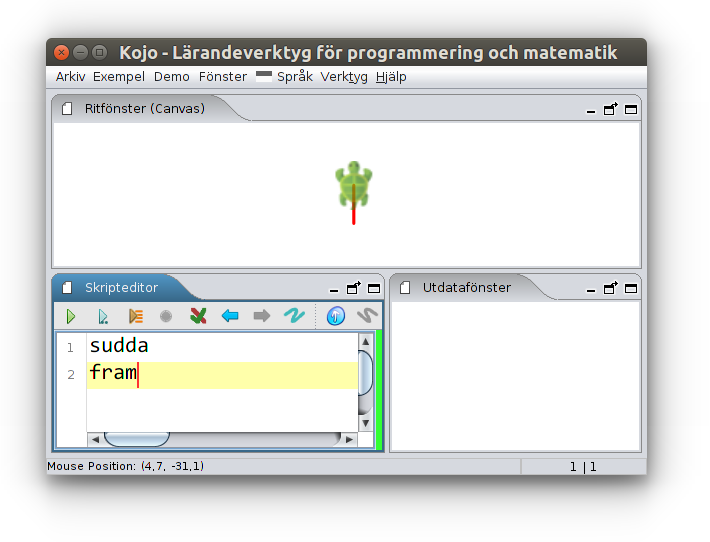
\includegraphics[width=14.0cm]{../img/kojo.png}
\end{center}

\end{multicols}

\chapter{Dein erstes Programm}
\begin{multicols}{2}
\section*{\color{BrickRed}Aufgabe:}
Schreibe diese Worte in Kojos Programmbearbeiter:

\begin{lstlisting}[basicstyle={\ttfamily\fontsize{30}{36}\selectfont},numbers=none]
leeren
vor
\end{lstlisting}
        
Klicke auf das grüne Ausführen-Symbol 

\includegraphics[width=1.0cm]{../img/play.png}
\\

um das Programm zu starten.
\\

\vskip 5.0em

\columnbreak

\begin{center}
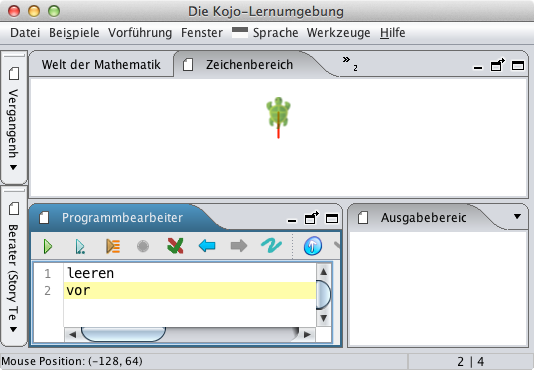
\includegraphics[width=14.0cm]{../img/fram_de.png}
\end{center}

\end{multicols}

\chapter{Zeichne ein Quadrat}
\begin{multicols}{2}

\begin{lstlisting}[basicstyle={\ttfamily\fontsize{30}{36}\selectfont},numbers=none]
leeren
vor
rechts
\end{lstlisting}
        
Bei Eingabe von \lstinline{links} oder \lstinline{rechts} dreht sich die Kröte.
\section*{\color{BrickRed}Aufgabe:}
Erweitere das Programm so, dass ein Quadrat gezeichnet wird.

\columnbreak

\begin{center}
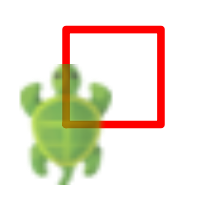
\includegraphics{../img/square.png}
\end{center}

\end{multicols}

\chapter{Zeichne eine Treppe}
\begin{multicols}{2}

\begin{lstlisting}[basicstyle={\ttfamily\fontsize{30}{36}\selectfont},numbers=none]
leeren
vor; links
vor; rechts
\end{lstlisting}
        
\vskip 1.0em
Mehrere Befehle in einer Zeile müssen durch ein Semikolon \lstinline{;} getrennt werden.
\section*{\color{BrickRed}Aufgabe:}
Erweitere das Programm so, dass eine Treppe gezeichnet wird.

\columnbreak

\begin{center}

\includegraphics{../img/stairs.png}
\end{center}

\end{multicols}

\chapter{Nutze eine Schleife}
\begin{multicols}{2}

\begin{lstlisting}[basicstyle={\ttfamily\fontsize{30}{36}\selectfont},numbers=none]
leeren
schleife(4){ vor; rechts }
\end{lstlisting}
        
Mit einer {\it Schleife} kannst Du Befehle wiederholt ausführen.
\section*{\color{BrickRed}Aufgabe:}


\begin{itemize}

\item {Was passiert, wenn Du statt 4 die Zahl 100 eingibst?}
\item {Zeichne eine Treppe mit 100 Stufen.}

\end{itemize}



\columnbreak

\begin{center}
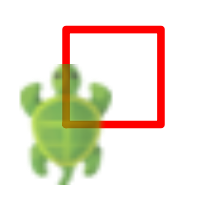
\includegraphics{../img/square.png}
\end{center}

\end{multicols}

\chapter{Übergebe Parameter}
\begin{multicols}{2}

\begin{lstlisting}[basicstyle={\ttfamily\fontsize{30}{36}\selectfont},numbers=none]
vor(40)
rechts(60)
links(40)
\end{lstlisting}
        
\vskip 1.0em
Du kannst Befehlen {\it Parameter} übergeben, damit sie nicht die Standardwerte verwenden.
\section*{\color{BrickRed}Aufgabe:}


\begin{itemize}

\item {Zeichne ein Vieleck}

\end{itemize}



\columnbreak

\begin{center}
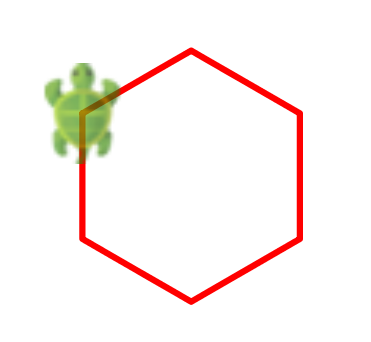
\includegraphics{../img/de/hexagon.png}
\end{center}

\end{multicols}

\chapter{Bewege Dich zum Ziel}
\begin{multicols}{2}

\begin{lstlisting}[basicstyle={\ttfamily\fontsize{30}{36}\selectfont},numbers=none]
springen
springen(90)
springen(100,200)
gehen(65,180)
\end{lstlisting}
        
\vskip 1.0em
Die Position der Maus im Zeichenbereich kannst Du links unter dem Programmbearbeiter ablesen:
\vskip 1.0em

\includegraphics[width=5.0cm]{../img/de/mousepos.png}
\section*{\color{BrickRed}Aufgabe:}


\begin{itemize}

\item {Zeichne ein Quadrat im Quadrat.}

\end{itemize}




\begin{itemize}

\item {Zeichne Diagonalen in das Quadrat.}

\end{itemize}



\columnbreak

\begin{center}
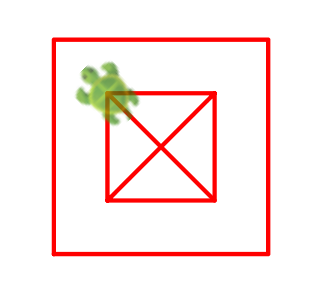
\includegraphics{../img/de/quadrate.png}
\end{center}

\end{multicols}

\chapter{Zeichne eine farbige Figur}
\begin{multicols}{2}

\begin{lstlisting}[basicstyle={\ttfamily\fontsize{25}{30}\selectfont},numbers=none]
schreiben("Mein Name ist...")
stiftfarbe(lila)
füllfarbe(grün)
\end{lstlisting}
        
\vskip 1.0em
\section*{\color{BrickRed}Aufgabe:}
Zeichne eine einfache farbige Figur.


\columnbreak


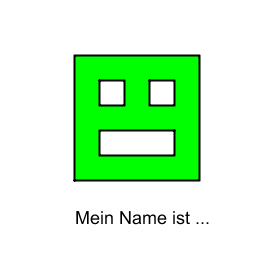
\includegraphics[width=5.0cm]{../img/de/head.png}
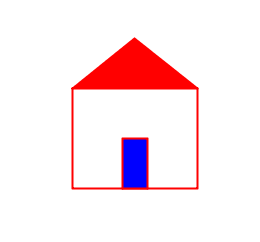
\includegraphics[width=6.0cm]{../img/de/house.png}
\end{multicols}

\chapter{Wie schnell ist Dein Computer?}Der erste Computer hieß {\bf ENIAC} und konnte in einer Sekunde bis 5000 zählen.\\
In Kojo gibt es eine Funktion \lstinline{zählzeitStoppen} die misst, wie schnell Dein Computer zählen kann.\\
Wenn ich \lstinline{zählzeitStoppen(5000)} ausführe, dann wird die Zeit ausgegeben, die mein Computer für das Zählen braucht:

\begin{lstlisting}[numbers=none]

*** Zählt von 1 bis ... 5000 *** FERTIG!
Es dauerte 0.32 Millisekunden.
      
\end{lstlisting}
        
\section*{\color{BrickRed}Aufgabe:}


\begin{itemize}

\item {Gib ein \lstinline{zählzeitStoppen(5000)} und prüfe, ob Dein Computer schneller ist als meiner.}
\item {Wie lange braucht Dein Computer, um bis eine Million zu zählen?}
\item {Wie weit kann Dein Rechner in einer Sekunde zählen?}

\end{itemize}


\chapter{Verfolge Dein Programm}
\begin{multicols}{2}
\section*{\color{BrickRed}Aufgabe:}


\begin{itemize}

\item {Schreibe ein Programm, das eine Stufe zeichnet.}
\item {Klicke auf das orange Verfolgen-Symbol.}
\item {Klicke auf einen der Aufrufe: \lstinline{CALL vor ()}. Was passiert im Zeichenbereich?}
\item {Im Programmbearbeiter wird der zugehörige Befehl blau markiert. Deaktiviere die Markierung, indem Du neben die Markierung klickst.}
\item {Füge dem Programm weitere Befehle hinzu und probiere aus, was passiert, wenn Du sie verfolgst}
\item {Schließe das Fenster {\it Programmschritte verfolgen} wenn Du fertig bist.}

\end{itemize}



\columnbreak

\begin{center}
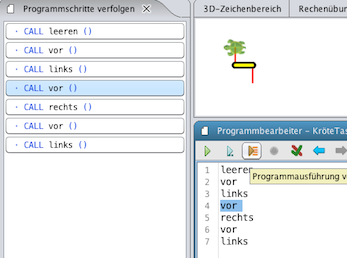
\includegraphics{../img/trace_de.png}
\end{center}

\end{multicols}

\chapter{Erstelle Deine eigene Funktion mit \lstinline{def}}Mit \lstinline{def} kannst Du einer eigenen {\it Funktion} einen Namen geben.

\begin{lstlisting}[basicstyle={\ttfamily\fontsize{20}{24}\selectfont},numbers=none]
def quadrat =  schleife(4){ vor; rechts }  

leeren
quadrat    //Ruft die Quadrat-Funktion auf.
springen
quadrat
\end{lstlisting}
        
\section*{\color{BrickRed}Aufgabe:}


\begin{itemize}

\item {Ändere die Farbe der Quadrate.}
\item {Erstelle mehr Quadrate.}

\end{itemize}


\section*{\color{OliveGreen}Tipps:}

\begin{lstlisting}[numbers=none]
füllfarbe(grün); stiftfarbe(lila)
\end{lstlisting}
        
\chapter{Stapel Quadrate}
\begin{multicols}{2}
\section*{\color{BrickRed}Aufgabe:}
Erstelle einen Stapel von 10 Quadraten.
\section*{\color{OliveGreen}Tipps:}
\vskip 1.0em

\begin{lstlisting}[numbers=none]
def quadrat =  schleife(4){ vor; rechts }  

leeren; langsam(100)
schleife(10){ ??? }
\end{lstlisting}
        

\columnbreak

\begin{center}
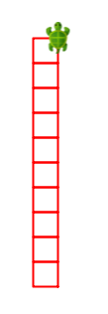
\includegraphics{../img/square-column.png}
\end{center}

\end{multicols}

\chapter{Schreibe eine Stapelfunktion}
\begin{multicols}{2}
\section*{\color{BrickRed}Aufgabe:}
Schreibe eine Funktion mit dem Namen \lstinline{stapel}, die einen Stapel aus 10 Quadraten zeichnet.
\section*{\color{OliveGreen}Tipps:}

\begin{lstlisting}[numbers=none]
def quadrat = schleife(4){ vor; rechts }  
def stapel = ???

leeren; langsam(100)
stapel
\end{lstlisting}
        

\columnbreak

\begin{center}
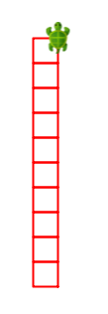
\includegraphics{../img/square-column.png}
\end{center}

\end{multicols}

\chapter{Erstelle ein Gitter}
\begin{multicols}{2}
\section*{\color{BrickRed}Aufgabe:}
Erstelle ein Gitter aus 10 * 10 Quadraten.
\section*{\color{OliveGreen}Tipps:}


\begin{itemize}

\item {Verwende hierfür Deine Stapelfunktion von eben.}
\item {Du kannst eine ganze Stapelhöhe zurück springen mit \lstinline{springen(-10 * 25)}}
\item {Du kannst dann an die richtige Stelle springen mit \lstinline{rechts; springen; links}}

\end{itemize}



\columnbreak

\begin{center}
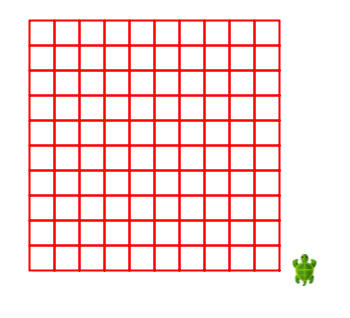
\includegraphics{../img/square-grid.png}
\end{center}

\end{multicols}

\chapter{Quadrat mit Parameter}
\begin{multicols}{2}
\section*{\color{BrickRed}Aufgabe:}
Zeichne verschiedene Quadrate.
\section*{\color{OliveGreen}Tipps:}
Gib Deiner Quadrat-Funktion einen {\it Parameter}\\
mit dem Namen \lstinline{seitenlänge} und Typ \lstinline{Ganzzahl}:

\begin{lstlisting}[basicstyle={\ttfamily\fontsize{16}{19}\selectfont},numbers=none]
def quadrat(seitenlänge : Ganzzahl) = 
  schleife(4){ vor(seitenlänge); rechts }

leeren; langsam(100); unsichtbar
quadrat(100) 
quadrat(70)
quadrat(40)
\end{lstlisting}
        
Du kannst die Farbe ändern mit:\\
\lstinline{füllfarbe(blau); stiftfarbe(rosa)}


\columnbreak


\begin{center}

\includegraphics[width=5.0cm]{../img/square-param.png}
\end{center}

\begin{center}

\includegraphics[width=5.0cm]{../img/square-param-color.png}
\end{center}

\end{multicols}

\chapter{Zeichne einen Quadratkopf}\section*{\color{BrickRed}Aufgabe:}
Zeichne einen Kopf aus verschiedenen Quadraten.
\\


\begin{tikzpicture}[overlay]
\node at (20.0cm,-1.0cm) {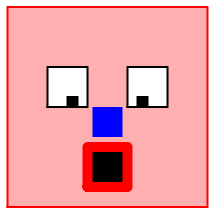
\includegraphics[width=5.5cm]{../img/square-man.png}};
\end{tikzpicture}
  
\section*{\color{OliveGreen}Tipps:}

\begin{lstlisting}[basicstyle={\ttfamily\fontsize{14}{17}\selectfont},numbers=none]
def quadrat(x: Ganzzahl, y: Ganzzahl, seitenlänge: Ganzzahl) = {
  springen(x, y)
  schleife(4) { vor(seitenlänge); rechts }
}
def kopf(x: Ganzzahl, y: Ganzzahl) = { füllfarbe(rosa); stiftfarbe(rot); quadrat(x, y, 200) }
def auge(x: Ganzzahl, y: Ganzzahl) = { füllfarbe(weiß); stiftfarbe(schwarz); quadrat(x, y, 40) }
def pupille(x: Ganzzahl, y: Ganzzahl) = { füllfarbe(schwarz); stiftfarbe(schwarz); quadrat(x, y, 10) }
def nase(x: Ganzzahl, y: Ganzzahl) = { füllfarbe(blau); stiftfarbe(durchsichtig); quadrat(x, y, 30) }
def mund(x: Ganzzahl, y: Ganzzahl) = { stiftbreite(10); füllfarbe(schwarz); 
                                            stiftfarbe(rot); quadrat(x, y, 40) }

leeren; langsam(20); unsichtbar
kopf(0, 0)
auge(40, 100); pupille(60, 100)
???
\end{lstlisting}
        
\chapter{Zeichne ein Vieleck}\section*{\color{BrickRed}Aufgabe:}


\begin{itemize}

\item {Probiere das Programm unten aus. Zeichne verschiedene Vielecke.}
\item {Füge einen Parameter \lstinline{seitenlänge} hinzu und zeichne verschieden große Vielecke.}
\item {Wie groß muss n sein, damit ein Kreis entsteht?}

\end{itemize}


\section*{\color{OliveGreen}Tipps:}

\begin{lstlisting}[basicstyle={\ttfamily\fontsize{18}{22}\selectfont},numbers=none]
def vieleck(n: Ganzzahl) = schleife(n){
  vor(100)
  links(360.0/n)
}

leeren; langsam(100)
vieleck(7)
\end{lstlisting}
        

\begin{tikzpicture}[overlay]
\node at (20.0cm,3.5cm) {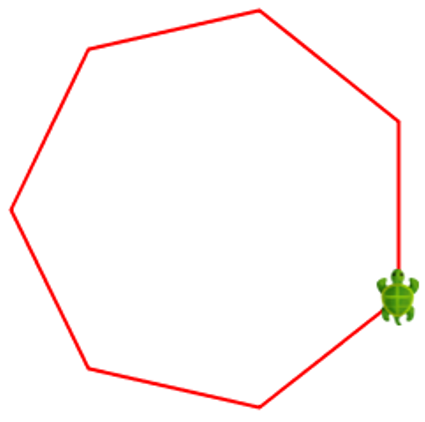
\includegraphics[width=8.0cm]{../img/polygon.png}};
\end{tikzpicture}
  
\chapter{Zeichne viele Vielecke}\section*{\color{BrickRed}Aufgabe:}


\begin{itemize}

\item {Probiere das Programm unten aus.}
\item {Verändere die Anzahl der Seiten und den Winkel.}
\item {Fülle die Vielecke mit Farbe.}

\end{itemize}



\begin{tikzpicture}[overlay]
\node at (22.0cm,-0.5cm) {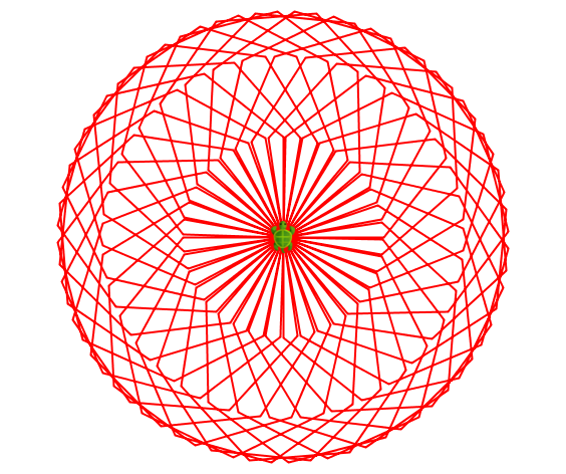
\includegraphics[width=11.0cm]{../img/polygons-circle.png}};
\end{tikzpicture}
  

\begin{lstlisting}[basicstyle={\ttfamily\fontsize{16}{19}\selectfont},numbers=none]
def vieleck(n: Ganzzahl, seitenlänge: Ganzzahl) = 
  schleife(n){
    vor(seitenlänge)
    links(360.0/n)
  }
def drehen(n: Ganzzahl, winkel: Ganzzahl, seitenlänge: Ganzzahl) = 
  schleife(360/winkel){ 
    vieleck(n, seitenlänge) 
    links(winkel) 
  }

leeren; langsam(5)
drehen(7, 10, 100)
\end{lstlisting}
        
\chapter{Werte und Ausdrücke}
\begin{multicols}{2}
\section*{\color{BrickRed}Aufgabe:}


\begin{itemize}

\item {Schreibe \lstinline{1 + 1} und klicke die blaue Ausführen-Taste. Dann erstellt Kojo einen grünen Kommentar.}
\item {Der Kommentar sagt, dass der Wert des Ausdrucks \lstinline{1 + 1} gleich \lstinline{2} ist und dass der Typ \lstinline{Int} ist. \lstinline{Int} ist eine Abkürzung für Integer, auf Deutsch: \lstinline{Ganzzahl}.}
\item {Führe weitere Berechnungen durch. Welcher Wert und Typ wird ausgegeben?}

\end{itemize}



\begin{lstlisting}[numbers=none]
5 * 5
10 + 2 * 5
"Auf" + " Wieder" + "sehen"
5 / 2
5 / 2.0
5 % 2
\end{lstlisting}
        


\columnbreak


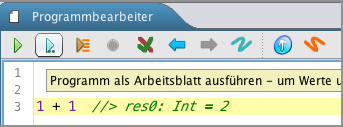
\includegraphics[width=12.0cm]{../img/show-value_de.png}
\section*{\color{OliveGreen}Tipps:}


\begin{itemize}

\item {Steht \lstinline{/} zwischen ganzen Zahlen, so wird eine ganzzahlige Division ausgeführt. Das heißt, die Nachkommastellen entfallen. Für eine Division mit Nachkommastellen muss mindestens eine Zahl eine Bruchzahl sein.}
\item {Mit \lstinline{%} erhältst Du den Rest einer ganzzahligen Division.}

\end{itemize}


\end{multicols}

\chapter{Gebe einem Wert einen Namen mit \lstinline{val}}
\begin{multicols}{2}
\section*{\color{BrickRed}Aufgabe:}
Mit \lstinline{val} kannst Du einen Namen mit einem Wert koppeln. Der Name kann dann anstelle des Wertes verwendet werden. Probiere das folgende Programm aus. Was schreibt die Kröte?

\begin{lstlisting}[numbers=none]
val x = 10
val y = 5
val gurke = x + y
val banane = x * y

leeren
vor; schreiben(banane)
vor; schreiben(gurke)
vor; schreiben(y)
vor; schreiben(x)
\end{lstlisting}
        

\columnbreak

\begin{center}
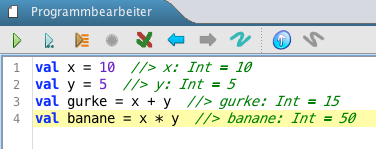
\includegraphics[width=12.0cm]{../img/val_de.png}
\end{center}

\end{multicols}

\chapter{Zufallszahlen}\section*{\color{BrickRed}Aufgabe:}


\begin{itemize}

\item {Führe das Programm unten mehrmals aus. Was passiert?}
\item {Was ist der kleinste und der größte mögliche Wert des Radius \lstinline{r}?}
\item {Ändere \lstinline{r} zu einer Zufallszahl zwischen 3 und 200.}
\item {Zeichne 100 Kreise mit zufälligem Radius und zufälliger Position wie im Bild rechts.}

\end{itemize}



\begin{tikzpicture}[overlay]
\node at (21.0cm,-5.0cm) {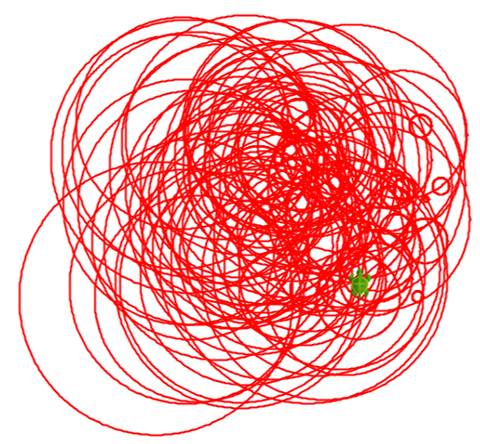
\includegraphics[width=8.0cm]{../img/random-circles.png}};
\end{tikzpicture}
  

\begin{lstlisting}[basicstyle={\ttfamily\fontsize{20}{24}\selectfont},numbers=none]
// zufall(90) liefert eine Zufallszahl zwischen 0 und 99:
val r = zufall(90) + 10   

leeren; langsam(10); unsichtbar
schreiben("Radius = " + r)
kreis(r)
\end{lstlisting}
        
\chapter{Mische Deine eigenen Farben}

\begin{itemize}

\item {Mit \lstinline{Color} kannst Du Deine eigenen Farben erstellen, z.B. \lstinline{Color(0, 70, 0)}}
\item {Die drei Parameter geben den Farbanteil von {\it rot}, {\it grün} und {\it blau} an.}
\item {Du kannst auch einen vierten Parameter für die {\it Deckkraft} angeben.}
\item {Alle Parameterwerte müssen zwischen 0 und 255 liegen.}

\end{itemize}


\section*{\color{BrickRed}Aufgabe:}
Probiere das folgende Programm. Ändere die Deckkraft.

\begin{tikzpicture}[overlay]
\node at (23.0cm,-2.0cm) {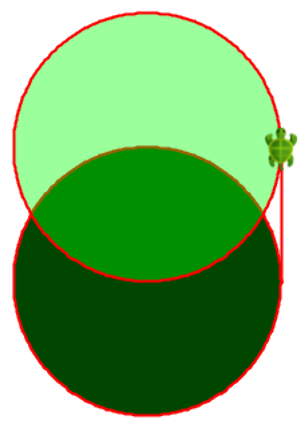
\includegraphics[width=7.0cm]{../img/color-circles.png}};
\end{tikzpicture}
  

\begin{lstlisting}[basicstyle={\ttfamily\fontsize{16}{19}\selectfont},numbers=none]
leeren; langsam(100)      

val olivgrün = Color(0,70,0)
val pistazie = Color(0,255,0,100)

füllfarbe(olivgrün); kreis(100)
füllfarbe(pistazie); vor(100); kreis(100)
\end{lstlisting}
        
\chapter{Probiere die Farbauswahl}
\begin{multicols}{2}
\section*{\color{BrickRed}Aufgabe:}


\begin{itemize}

\item {Mache einen Rechtsklick im Programmbearbeiter und gehe auf \lstinline{Farbe auswählen...}}
\item {Unter {\bf RGB} kannst Du eine neue RGB-Farbe mischen.}
\item {Drücke OK und schaue in den Ausgabebereich. Hier werden die RGB-Werte für Rot, Grün und Blau angezeigt.}
\item {Du kannst diese Werte verwenden, um mit der ausgewählten Farbe zu zeichnen \lstinline{stiftfarbe(Color(218, 103, 67))}.}

\end{itemize}



\columnbreak

\begin{center}
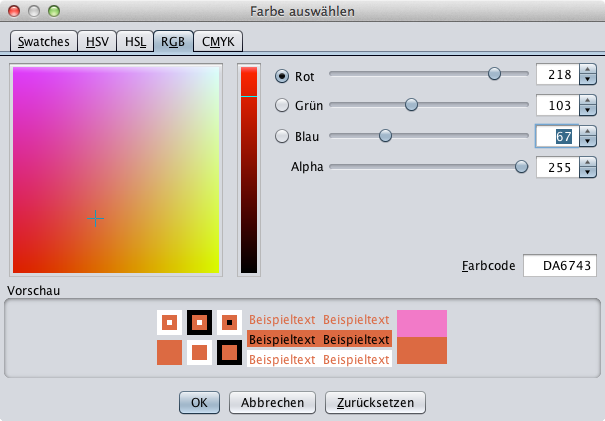
\includegraphics[width=12.0cm]{../img/color-chooser-rgb_de.png}
\end{center}

\end{multicols}

\chapter{Zeichne Zufallskreise}
\begin{multicols}{2}

\begin{lstlisting}[basicstyle={\ttfamily\fontsize{16}{19}\selectfont},numbers=none]
def zufällig = zufall(256)
def zufallsfarbe = 
       Color(zufällig,10, zufällig,100) 

leeren; langsam(5)
grundfarbeUO(schwarz,weiß)
stiftbreite(6)

schleife(100) {
    stiftfarbe(zufallsfarbe)
    kreis(100)
    springen(20)
    rechts(35)
}
\end{lstlisting}
        
\section*{\color{BrickRed}Aufgabe:}
Probiere verschiedene zufällige Stift- und Hintergrund-Farben aus.


\columnbreak


\begin{center}
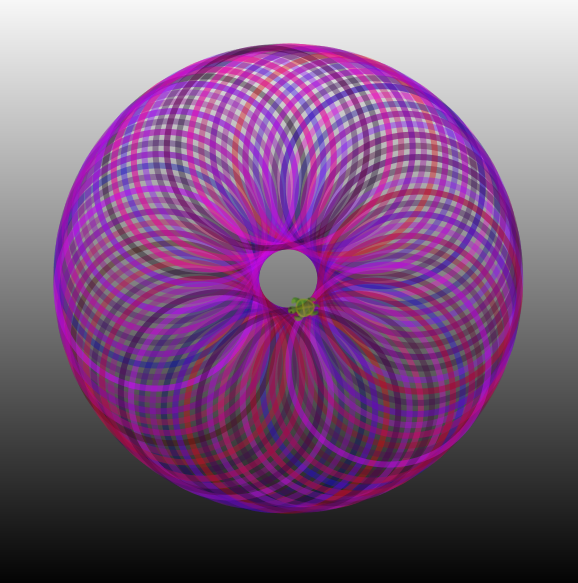
\includegraphics[width=12.0cm]{../img/circle-of-circles.png}
\end{center}

\end{multicols}

\chapter{Zeichne eine Blume}\section*{\color{BrickRed}Aufgabe:}
Das folgende Programm zeichnet 100 Kreise mit zufälliger Farbe, zufälligem Radius und zufälliger Ausrichtung. Probiere verschiedene Zufallszahlen-Grenzen und versuche zu erklären, was hierbei passiert.

\begin{tikzpicture}[overlay]
\node at (22.0cm,-4.0cm) {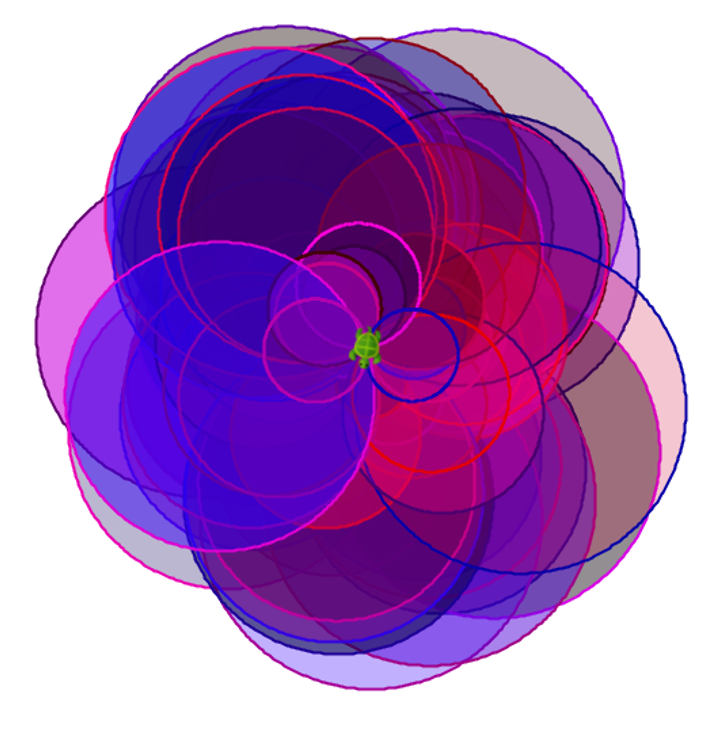
\includegraphics[width=8.5cm]{../img/random-color-circles.png}};
\end{tikzpicture}
  

\begin{lstlisting}[basicstyle={\ttfamily\fontsize{16}{19}\selectfont},numbers=none]
leeren(); langsam(5)
stiftbreite(2)
schleife(100){
  stiftfarbe(Color(zufall(256),0,zufall(256)))
  füllfarbe(Color(zufall(256),0,zufall(256),zufall(100)+50))
  links(zufall(360))
  kreis(zufall(30)*4+10)
}
\end{lstlisting}
        
\chapter{Erstelle eine Variable mit \lstinline{var}}Mit \lstinline{var} kannst Du einen Namen mit einem Wert koppeln.\\
Einer Variablen kann man jederzeit einen neuen Wert zuweisen:

\begin{lstlisting}[numbers=none]

var gurke = 1
gurke = 1 + 1   //erst wird 1 + 1 ausgerechnet, gurke bekommt dann den Wert 2        
        
\end{lstlisting}
        
\section*{\color{BrickRed}Aufgabe:}
Probiere das Programm aus. Was schreibt die Kröte?

\begin{lstlisting}[basicstyle={\ttfamily\fontsize{14}{17}\selectfont},numbers=none]
var i = 0

leeren
schleife(10){
  i = i + 1
  vor; schreiben(i)
}
\end{lstlisting}
        
\section*{\color{OliveGreen}Tipps:}


\begin{itemize}

\item {Die Zuweisung \lstinline{i = i + 1} weist \lstinline{i} einen neuen Wert zu, der sich aus dem {\it alten} Wert von \lstinline{i} plus \lstinline{1} berechnet.}

\end{itemize}


\chapter{Zeichne viele Blumen}\section*{\color{BrickRed}Aufgabe:}


\begin{itemize}

\item {Schreibe eine Funktion mit dem Namen \lstinline{blume}, die eine Blüte zeichnet und einen Stiel mit einem grünen Blatt, der in der Mitte der Blüte beginnt.}
\item {Zeichne 5 Blumen nebeneinander.}

\end{itemize}



\begin{tikzpicture}[overlay]
\node at (15.0cm,-7.0cm) {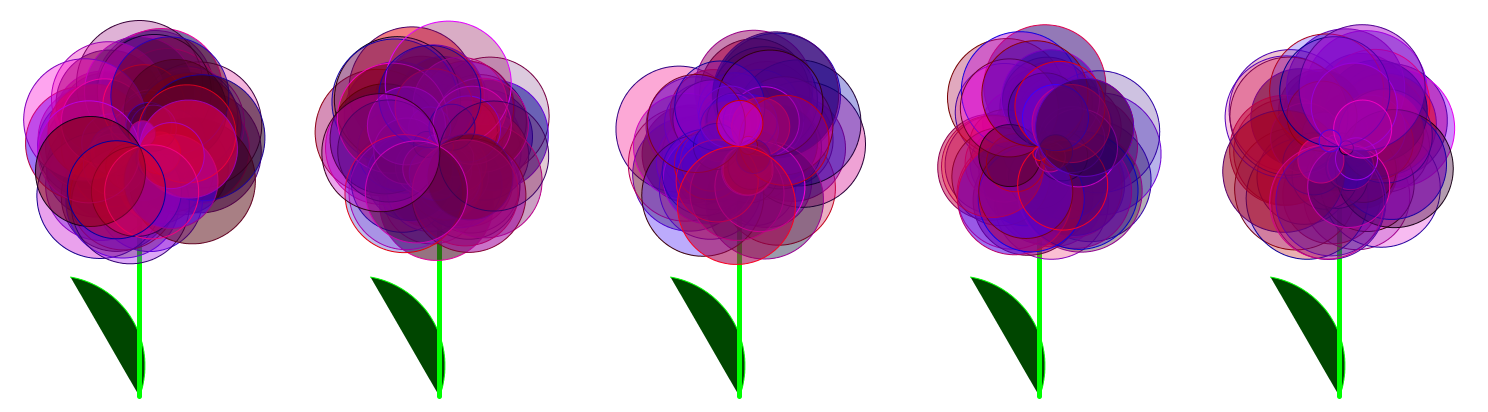
\includegraphics[width=16.0cm]{../img/flowers.png}};
\end{tikzpicture}
  
\section*{\color{OliveGreen}Tipps:}
Du kannst die Blätter zeichnen mit \lstinline{bogen(radius, winkel)}. \\
Gib der Funktion \lstinline{blume} zwei Parameter x und y und benutze \lstinline{springen(x,y)}\\
Du kannst die Schleife fünfmal ausführen und die Position wie folgt ausrechnen:

\begin{lstlisting}[basicstyle={\ttfamily\fontsize{18}{22}\selectfont},numbers=none]
var i = 0          
schleife(5){
  blume(600*i,0)
  i = i + 1        
}
\end{lstlisting}
        
\chapter{Gebe der Kröte ein neues Kostüm}\section*{\color{BrickRed}Aufgabe:}
Lade die Mediendateien von Kojos Webseite:
\href{http://www.kogics.net/kojo-download#media}{www.kogics.net/kojo-download\#media}


\begin{itemize}

\item {Entpacke die Datei \lstinline{scratch-media.zip} und finde das Krabbenbild \lstinline{crab1-b.png} im Ordner \lstinline{Media/Costumes/Animals}}
\item {Speichere die Datei \lstinline{crab1-b.png} in dem Ordner, in dem auch das Programm liegt.}
\item {Ziehe der Kröte ein Krabbenkostüm an:}

\end{itemize}



\begin{tikzpicture}[overlay]
\node at (12.0cm,-2.5cm) {
\includegraphics[width=3.0cm]{../img/crab1-b.png}};
\end{tikzpicture}
  

\begin{lstlisting}[basicstyle={\ttfamily\fontsize{12}{15}\selectfont},numbers=none]
leeren
kostüm("crab1-b.png")  
langsam(2000)
vor(1000)
\end{lstlisting}
        
\section*{\color{OliveGreen}Tipps:}


\begin{itemize}

\item {Du kannst auch eigene Bilder vom Typ \lstinline{.png} oder \lstinline{.jpg} verwenden.}
\item {Wenn Du das Bild in einem anderen Ordner speichern wilst, musst Du den Dateipfad angeben, z.B. \lstinline{kostüm("~/Kojo/Media/Costumes/Animals/crab1-b.png")}. Das Zeichen \lstinline{~} steht für Dein Home-Verzeichnis.}

\end{itemize}


\chapter{Erstelle weitere Kröten mit \lstinline{new}}Du kannst viele neue Kröten mit \lstinline{new} hinzufügen:

\begin{lstlisting}[basicstyle={\ttfamily\fontsize{18}{22}\selectfont},numbers=none]
leeren
val k1 = new Kröte(100,100)  //die neue Kröte k1 startet auf der Position (100, 100)
val k2 = new Kröte(100, 50)  //die neue Kröte k2 startet auf der Position (100, 50)
k1.vor(100)
k2.rück(100)  //Kröte k2 nach unten
\end{lstlisting}
        

\begin{tikzpicture}[overlay]
\node at (22.0cm,-2.0cm) {
\includegraphics[width=5.0cm]{../img/new.png}};
\end{tikzpicture}
  
\section*{\color{BrickRed}Aufgabe:}


\begin{itemize}

\item {Erzeuge drei Kröten übereinander.}
\item {Alle drei sollen nach links schauen.}

\end{itemize}


\section*{\color{OliveGreen}Tipps:}


\begin{itemize}

\item {\lstinline{k1} und \lstinline{k2} sind die {\it Namen} der neuen Kröten. Du kannst die Namen ändern, wenn Du willst.}
\item {Mit \lstinline{k1} gefolgt von einem Punkt kannst Du der Kröte k1 einen Befehl geben: \lstinline{k1.links}}
\item {Mit dem Befehl \lstinline{unsichtbar} kannst Du eine Kröte verbergen.}

\end{itemize}


\chapter{Krötenrennen}
\begin{multicols}{2}
Mit Hilfe von Zufallszahlen kannst Du die Kröten um die Wette rennen lassen.
\section*{\color{BrickRed}Aufgabe:}


\begin{itemize}

\item {Lass die drei Kröten laufen.}
\item {Wenn alle Kröten 10 mal nach vorn laufen, welche Kröte ist dann die Erste?}

\end{itemize}


\section*{\color{OliveGreen}Tipps:}


\begin{itemize}

\item {Mit \lstinline{k1.vor(zufall(100) + 1)} bewegt sich k1 zwischen 1 und 100 Schritten weit.}

\end{itemize}



\columnbreak

\begin{center}
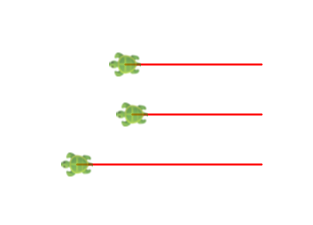
\includegraphics[width=12.0cm]{../img/race.png}
\end{center}

\end{multicols}

\chapter{Alternative mit \lstinline{if}}Mit einer \lstinline{if}-Anweisung kann man den Computer aufgrund einer Bedingung zwischen zwei Alternativen wählen lassen.

\begin{lstlisting}[basicstyle={\ttfamily\fontsize{20}{24}\selectfont},numbers=none]
leeren; unsichtbar
if (true) schreiben("wahr") else schreiben("falsch")
\end{lstlisting}
        
\section*{\color{BrickRed}Aufgabe:}


\begin{itemize}

\item {Ändere die Bedingung \lstinline{true} in \lstinline{false} und prüfe, was die Kröte schreibt.}
\item {Ändere die Bedingung in \lstinline{2 > 1} und prüfe, was die Kröte schreibt.}
\item {Ändere die Bedingung in \lstinline{2 < 1} und prüfe, was die Kröte schreibt.}
\item {Erkläre wie eine \lstinline{if}-Anweisung funktioniert.}

\end{itemize}


\section*{\color{OliveGreen}Tipps:}


\begin{itemize}

\item {Hinter \lstinline{if} kommt immer eine Bedingung in Klammern.}
\item {Wenn die Bedingung nach dem \lstinline{if} gleich \lstinline{true} ist, wird der Befehl hinter der Bedingung ausgeführt.}
\item {Wenn die Bedingung nach dem \lstinline{if} gleich \lstinline{false} ist, wird der Befehl hinter \lstinline{else} ausgeführt.}

\end{itemize}


\chapter{Reagiere auf das, was der Nutzer macht}
\begin{lstlisting}[basicstyle={\ttfamily\fontsize{20}{24}\selectfont},numbers=none]
ausgabeLeeren; setOutputTextFontSize(35)
val passwort = "gurke"
val frage     = "Wie lautet mein Passwort?"
val richtig      = "Der Safe ist offen!"
val fehler       = "Du kommst nicht hinein!"
val antwort = einlesen(frage)  //Warten auf die Antwort des Nutzers
val meldung = if (antwort == passwort) richtig else fehler
ausgeben(meldung)
\end{lstlisting}
        
\section*{\color{BrickRed}Aufgabe:}


\begin{itemize}

\item {Probiere das Programm aus. Du musst im Ausgabebereich unten etwas eingeben und mit der Eingabetaste bestätigen. Erkläre, was passiert.}
\item {Ändere das Passwort. Was wird ausgegeben, wenn man es richtig und wenn man es falsch eingibt?}
\item {Frage auch nach einem Benutzernamen und gib den Namen aus.}

\end{itemize}


\chapter{Nutze eine \lstinline{Solange}-Schleife}Mit \lstinline{schleifeSolange} wiederholt der Computer Anweisungen so lange, wie eine Bedingung wahr ist.

\begin{lstlisting}[basicstyle={\ttfamily\fontsize{22}{27}\selectfont},numbers=none]
leeren; unsichtbar; langsam(250); ausgabeLeeren
var x = 200
schleifeSolange (x > 0) {  //prüfe die Bedingung vor jeder Wiederholung 
  vor(x); rechts
  schreiben(x) 
  x = x - 12
}
ausgeben("x ist jetzt: " + x)
\end{lstlisting}
        
\section*{\color{BrickRed}Aufgabe:}


\begin{itemize}

\item {Was wird im Ausgabebereich ausgegeben? Warum?}
\item {Starte das Programm mit dem orangen Verfolgen-Symbol und prüfe jeden Schritt.}
\item {Ziehe statt \lstinline{12} den Wert \lstinline{20} von der Variablen \lstinline{x} ab. Erkläre, was passiert.}

\end{itemize}


\chapter{Zahlenraten}
\begin{lstlisting}[basicstyle={\ttfamily\fontsize{16}{19}\selectfont},numbers=none]
val geheimnis = zufall(100)+1
var antwort = einlesen("Rate eine Zahl zwischen 1 und 100! ")
var überspringen = true

schleifeSolange (überspringen) {
    if (antwort.toInt < geheimnis)
      antwort = einlesen(antwort + " ist zu KLEIN, rate erneut!")
    else if (antwort.toInt > geheimnis)
      antwort = einlesen(antwort + " ist zu GROSS, rate erneut!")
    else if (antwort.toInt == geheimnis)
      überspringen = false
}
ausgeben(geheimnis + " ist die RICHTIGE Antwort!")
\end{lstlisting}
        
\section*{\color{BrickRed}Aufgabe:}
Führe eine Variable \lstinline{var anzahlVersuche = 0} ein und stelle sicher, dass am Ende ausgegeben wird:\\
\lstinline{Richtige Antwort! Du hast es mit 5 Versuchen geschafft}
\chapter{Übe Multiplikation}
\begin{lstlisting}[basicstyle={\ttfamily\fontsize{16}{19}\selectfont},numbers=none]
var anzahlRichtig = 0
val startZeit = System.currentTimeMillis / 1000
schleife(12) {
  val zahl1 = zufall(12)+1
  val zahl2 = zufall(12)+1
  val antwort = einlesen("Was ist " + zahl1 + "*" + zahl2 + "?")
  if (antwort == (zahl1 * zahl2).toString) {
    ausgeben("Richtig!")
    anzahlRichtig = anzahlRichtig + 1
  }
  else ausgeben("Falsch. Die richtige Antwort ist " + (zahl1 * zahl2))
}
val stoppZeit = System.currentTimeMillis / 1000
val sekunde = stoppZeit - startZeit
ausgeben("Du hast " + anzahlRichtig + " richtige Antworten in " + sekunde + " Sekunden.")
\end{lstlisting}
        
\section*{\color{BrickRed}Aufgabe:}
Ändere das Programm so, dass man nur noch die Multiplikation mit 8 und 9 üben muss.
\chapter{Speichere Tiere in einem Vektor}
\begin{lstlisting}[basicstyle={\ttfamily\fontsize{14}{17}\selectfont},numbers=none]
var tiere = Vector("Elch", "Kuh", "Kaninchen", "Möve")  //Variable tiere enthält einen Vektor mit 4 Tieren
ausgeben("Das erste Tier im Vektor ist: " + tiere(0))     //Nummerierung der Werte im Vektor beginnt bei 0
ausgeben("Ein anderes Tier im Vektor ist:  " + tiere(1))
ausgeben("Der Vektor enthält so viele Tiere: " + tiere.size)
ausgeben("Das letzte Tier im Vektor ist:  " + tiere(tiere.size-1))

val s = zufall(tiere.size)   //berechnet eine Zufallszahl zwischen 0 und der Anzahl der Tiere minus 1
ausgeben("Ein zufälliges Tier: " + tiere(s))

tiere = tiere :+ "Kamel"    //fügt das Tier am Ende des Vektors ein
tiere = "Dromedar" +: tiere //fügt das Tier am Anfang des Vektors ein
tiere = tiere.updated(2, "Nilpferd")  //Ändert das dritte Tier (Nummer 2 im Vektor)
ausgeben("Alle Tiere rückwärts:")
tiere.foreach{ x => ausgeben(x.reverse) } //für alle x im Vektor: gebe x rückwärts aus
\end{lstlisting}
        
\section*{\color{BrickRed}Aufgabe:}


\begin{itemize}

\item {Was gibt das Programm im Ausgabebereich aus? Erkläre was passiert.}
\item {Füge dem Vektor ein weiteres Tier hinzu.}

\end{itemize}


\chapter{Übe Vokabeln}
\begin{lstlisting}[basicstyle={\ttfamily\fontsize{14}{17}\selectfont},numbers=none]
val deutsch = Vector("Rechner", "Schildkröte", "Kreis")
val englisch = Vector("computer", "turtle", "circle")
var anzahlRichtig = 0
schleife(5) {
  val i = zufall(deutsch.size)
  val vokabel = deutsch(i)
  val antwort = einlesen("Was heisst " + vokabel + " auf Englisch?")
  if (antwort == englisch(i)) {
    ausgeben("Richtige Antwort!")
    anzahlRichtig = anzahlRichtig + 1
  } else {
    ausgeben("Falsche Antwort. Die richtige Antwort lautet: " + englisch(i))
  }
}
ausgeben("Du hast " + anzahlRichtig + " richtige Antworten gegeben.")
\end{lstlisting}
        
\section*{\color{BrickRed}Aufgabe:}


\begin{itemize}

\item {Füge mehr Vokabeln ein.}
\item {Übe die Übersetzung vom Englischen ins Deutsche.}
\item {Lasse den Nutzer einstellen, wie viele Vokabeln er üben will. Tipp: \lstinline{val anzahl = einlesen("Gebe die Anzahl ein:").toInt}}

\end{itemize}


\chapter{Hauptstadt-Spiel}
\begin{lstlisting}[basicstyle={\ttfamily\fontsize{13}{16}\selectfont},numbers=none]
def hauptstadtSpiel = {
  ausgeben("Willkommen zum Hauptstadt-Spiel!")
  //Eine Map ist eine Abbildung, hier von Landesnamen zu Hauptstadtnamen:
  val stadt = Map("Schweden" ->"Stockholm", "Frankreich" -> "Paris", "Spanien" -> "Madrid")
  var länder = stadt.keySet //keySet liefert die Menge aller Schlüssel in einer Map 
  def zufallsLand = scala.util.Random.shuffle(länder.toVector).head
  schleifeSolange(!länder.isEmpty) {
    val land = zufallsLand
    val antwort = einlesen("Was ist die Hauptstadt von " + land + "?")
    ausgeben(s"Du sagst: $antwort")
    if (antwort == stadt(land)) {
      länder = länder - land  //entfernt das Land aus der Menge der Länder
      ausgeben("Richtig! Du hast noch " + länder.size + " Länder!")
    } else ausgeben(s"Falsch! Die Hauptstadt von $land beginnt mit ${stadt(land).take(2)}...")
  }
  ausgeben("DANKE FÜR DIE TEILNAHME! (Drücke ESC)")
}

toggleFullScreenOutput;  
setOutputBackground(black); setOutputTextColor(green); setOutputTextFontSize(30)
schleife(100)(ausgeben()) //fülle den Ausgabebereich mit 100 Leerzeilen
hauptstadtSpiel
//AUFGABE: Lege mehr Paare Land -> Stadt an. Messe die Zeit und zähle die Punkte.
\end{lstlisting}
        
\chapter{Erstelle eine Stoppuhr mit \lstinline{object}}
\begin{lstlisting}[basicstyle={\ttfamily\fontsize{14}{17}\selectfont},numbers=none]
object Stoppuhr {
  def jetzt = System.currentTimeMillis  //liefert die aktuelle Zeit in Millisekunden
  var zeit = jetzt
  def rücksetzen = { zeit = jetzt }
  def gemessen = jetzt - zeit
  def zufallsWarten(min: Int, max: Int) =  //wartet zwischen min und max Sekunden
    Thread.sleep((zufall(max-min)+min)*1000)  //Thread.sleep(1000) wartet 1 Sekunde
}

ausgeben("Klicke in den Ausgabebereich und warte...")
Stoppuhr.zufallsWarten(3, 6)   //wartet zwischen 3 und 6 Sekunden
Stoppuhr.rücksetzen
einlesen("Drücke die Eingabetaste, so schnell wie Du kannst.")
ausgeben("Reaktionszeit: " + (Stoppuhr.gemessen/1000.0) + " Sekunden")
\end{lstlisting}
        
Mit \lstinline{object} kannst Du alles sammeln, was zu einem Objekt gehört.\\
Du kannst mit einem Punkt auf etwas im Objekt zugreifen: \lstinline{Stoppuhr.rücksetzen}
\section*{\color{BrickRed}Aufgabe:}


\begin{itemize}

\item {Probiere das Programm aus und messe Deine Reaktionszeit. Wie schnell bist Du?}
\item {Nutze \lstinline{Stoppuhr} in der Aufgabe {\it Zahlenraten} und füge die folgende Ausgabe hinzu: \lstinline{Richtig geraten! Du hast es mit 5 Versuchen in 32 Sekunden geschafft}}

\end{itemize}


\chapter{Simuliere eine Ampel}
\begin{tikzpicture}[overlay]
\node at (22.0cm,-6.0cm) {
\includegraphics[width=3.0cm]{../img/traffic-lights.png}};
\end{tikzpicture}
  

\begin{lstlisting}[basicstyle={\ttfamily\fontsize{14}{17}\selectfont},numbers=none]
def alleLöschen = draw(penColor(gray) * fillColor(black) -> PicShape.rect(130,40))
def licht(c: Color, h: Int) = penColor(noColor) * fillColor(c) * trans(20,h) -> PicShape.circle(15)
def leuchtetRot = draw(licht(red, 100))
def leuchtetGelb = draw(licht(yellow, 65))
def leuchtetGrün = draw(licht(green, 30))
def warte(sekunden: Int) = Thread.sleep(sekunden*1000)

leeren; unsichtbar  
schleifeSolange (true) { //eine unendliche Schleife
  alleLöschen
  leuchtetRot;  warte(3)
  leuchtetGelb; warte(1) 
  alleLöschen
  leuchtetGrün; warte(3)
  leuchtetGelb; warte(1)
}
\end{lstlisting}
        
\section*{\color{BrickRed}Aufgabe:}


\begin{itemize}

\item {Wie wechselt die Ampel? Versuche zu erklären, was hierbei passiert.}
\item {Ändere das Programm so, dass die Ampel doppelt so lang auf grün bleibt.}

\end{itemize}


\chapter{Steuere die Kröte mit der Tastatur}
\begin{multicols}{2}

\begin{lstlisting}[basicstyle={\ttfamily\fontsize{18}{22}\selectfont},numbers=none]
leeren; langsam(0)
activateCanvas()

animate { vor(1) }

onKeyPress {
  case Kc.VK_LEFT  => links(5)
  case Kc.VK_RIGHT => rechts(5)
  case Kc.VK_SPACE => vor(5)
  case t => 
    ausgeben("Unbekannte Taste: " + t)
}
\end{lstlisting}
        


\columnbreak


\section*{\color{BrickRed}Aufgabe:}


\begin{itemize}

\item {Schreibe \lstinline{Kc.} und drücke \lstinline{Strg+Alt+Leertaste}. Dann kannst Du sehen, wie die verschiedenen Tasten heißen.}
\item {Befehle \lstinline{stiftRauf} wenn man Pfeil nach oben drückt}
\item {Befehle \lstinline{stiftRunter} wenn man Pfeil nach unten drückt}
\item {Befehle \lstinline{stiftfarbe(blau)} wenn man B drückt}
\item {Befehle \lstinline{stiftfarbe(rot)} wenn man R drückt}
\item {Erhöhe bzw. Verringere die Geschwindigkeit mit den Tasten + bzw. -}

\end{itemize}


\end{multicols}

\chapter{Steuere die Kröte mit der Maus}
\begin{multicols}{2}

\begin{lstlisting}[basicstyle={\ttfamily\fontsize{16}{19}\selectfont},numbers=none]
leeren; langsam(100)
activateCanvas()

var zeichnen = true

onKeyPress {
  case Kc.VK_DOWN =>
    stiftRunter()
    zeichnen = true
  case Kc.VK_UP =>
    stiftRauf()
    zeichnen = false
  case t =>
    ausgeben("Unbekannte Taste: " + t)
}

onMouseClick { (x, y) =>
  if (zeichnen) gehen(x, y) else springen(x, y)
}
\end{lstlisting}
        


\columnbreak


\section*{\color{BrickRed}Aufgabe:}


\begin{itemize}

\item {Befehle \lstinline{füllfarbe(schwarz)} wenn man F drückt}
\item {Führe die Variable \lstinline{var füllen = true} ein und mache bei Taste \lstinline{Kc.VK_F}:}

\end{itemize}



\begin{lstlisting}[numbers=none]

      if (füllen) {
        füllfarbe(schwarz)
        füllen=false
      } else {
        füllfarbe(durchsichtig)
        füllen=true
      }
      
\end{lstlisting}
        
\end{multicols}

\chapter{Erstelle Dein eigenes Bankkonto}
\begin{multicols}{2}

\begin{lstlisting}[basicstyle={\ttfamily\fontsize{16}{19}\selectfont},numbers=none]
object meinKonto {
  val nummer = 123456
  var stand = 0.0
  def einzahlen(betrag: Bruchzahl) = {
    stand = stand + betrag
  }
  def abheben(betrag: Bruchzahl) = {
    stand = stand - betrag
  }
  def anzeigen() = {
    ausgeben("Kontonummer: " + nummer)
    ausgeben(" Kontostand: " + stand)
  }
}

meinKonto.anzeigen()
meinKonto.einzahlen(100)
meinKonto.anzeigen()
meinKonto.abheben(10)
meinKonto.anzeigen()
\end{lstlisting}
        


\columnbreak


\section*{\color{BrickRed}Aufgabe:}


\begin{itemize}

\item {Was ist der Kontostand nach Ausführung des Programms? Erkläre was passiert.}
\item {Sorge mit \lstinline{if} dafür, dass nicht mehr Geld abgehoben werden kann, als auf dem Konto ist.}
\item {Lege eine Konstante \lstinline{val maxBetrag = 5000} an und sorge mit \lstinline{if} dafür, dass man nicht mehr abheben darf als \lstinline{maxBetrag}.}

\end{itemize}


\end{multicols}

\chapter{Erstelle viele Objekte mit \lstinline{class}}
\begin{multicols}{2}
Wenn Du viele verschiedene Konten erstellen willst, benötigst Du eine Klasse. Mit \lstinline{new} kannst Du davon neue Objekte erstellen. Jedes Objekt erhält eine eigene Kontonummer und Kontostand.

\begin{lstlisting}[basicstyle={\ttfamily\fontsize{13}{16}\selectfont},numbers=none]
class Konto(nummer: Ganzzahl) {
  private var stand = 0.0 //private bedeutet "versteckt"  
  def einzahlen(betrag: Bruchzahl) = {
    stand = stand + betrag 
  }
  def abheben(betrag: Bruchzahl) = { 
    stand = stand - betrag 
  }
  def anzeigen() = 
    ausgeben(s"Konto $nummer: $stand")
}

val konto1 = new Konto(12345) //neues Objekt erstellen
val konto2 = new Konto(67890) //Noch ein Objekt

konto1.einzahlen(99)
konto2.einzahlen(88)
konto1.abheben(57)
konto1.anzeigen
konto2.anzeigen
\end{lstlisting}
        


\columnbreak


\section*{\color{BrickRed}Aufgabe:}


\begin{itemize}

\item {Was ist der Stand der beiden Konten, nachdem das Programm ausgeführt wurde? Erkläre was passiert.}
\item {Erstelle weitere Konto-Objekte und zahle Beträge ein und hebe Beträge ab.}
\item {Füge einen Klassenparameter \lstinline{name: Text} hinzu, der den Namen des Kontoinhabers aufnehmen soll, wenn Objekte erstellt werden.}
\item {Sorge dafür, dass auch \lstinline{name} ausgegeben wird, wenn \lstinline{anzeigen} ausgeführt wird.}
\item {Was passiert, wenn Du das befiehlst: \lstinline{konto1.stand = 10000000 } ?}

\end{itemize}


\end{multicols}

\chapter{Sprich mit Deinem Computer}
\begin{lstlisting}[basicstyle={\ttfamily\fontsize{13}{16}\selectfont},numbers=none]
setOutputBackground(black); setOutputTextFontSize(30); setOutputTextColor(green)
ausgeben("Schreibe interessante Antworten, auch wenn die Fragen seltsam sind. Verabschiede Dich mit 'Tschüss'")
def zufällig(xs: Vector[String]) = scala.util.Random.shuffle(xs).head
val aufforderung = Vector("Was bedeutet", "Gefällt Dir", "Wozu brauchen wir", "Erzähl mir mehr über")
var antwort = "?"
val eröffnung = "Worüber möchtest Du reden?"
var worte = Vector("Nabelschnur", "Ketchupeis", "Weihnachtsmann", "Kissenbezüge")
schleifeSolange(antwort != "tschüss") {
  val t = if (antwort == "?") eröffnung
  else if (antwort == "nein") "Nee."
  else if (antwort == "ja") "Nun ja."
  else if (antwort.length < 4) "Oh..."
  else zufällig(aufforderung) + " " + zufällig(worte) + "?"
  antwort = einlesen(t).toLowerCase
  worte = worte ++ antwort.split("[ ,;:.!?]").toList.filter(_.length > 3)
}
ausgeben("Danke für das Gespräch! Jetzt habe ich diese Worte gelernt: " + worte)

//Aufgabe:
// (1) Probiere das Programm aus und versuche herauszufinden, wie es funktioniert.
// (2) Wann wird die Solange-Schleife beendet?
// (3) Fülle weitere Sätze und Worte in die Vektoren aufforderung und worte.
// (4) Erweitere die Reaktion auf kurze Antworten über "nein" und "ja" hinaus.
\end{lstlisting}
        
\chapter{Verändere das Tischtennis-Spiel}
\begin{multicols}{2}
\section*{\color{BrickRed}Aufgabe:}


\begin{itemize}

\item {Wähle im Menü Beispiele > Animationen und Spiele > Tischtennis. Probiere es aus!}
\item {Du kannst es steuern mit: Pfeil nach oben/unten und A/Z.}
\item {Drücke ESC um das Spiel zu beenden und untersuche das Programm. Es nutzt die englischen Kojo-Befehle.}
\item {Ändere das Programm so, dass man mit Y statt Z den linken Schläger nach unten bewegen kann. Dann ist das Spiel bei einer deutschen Tastatur bequemer für den linken Spieler.}
\item {Ändere das Programm so, dass der Ball größer wird.}
\item {Ändere das Spielfeld zu einem Tennistisch mit grünem Hintergrund, weißen Linien und einem gelben Ball.}

\end{itemize}



\columnbreak

\begin{center}
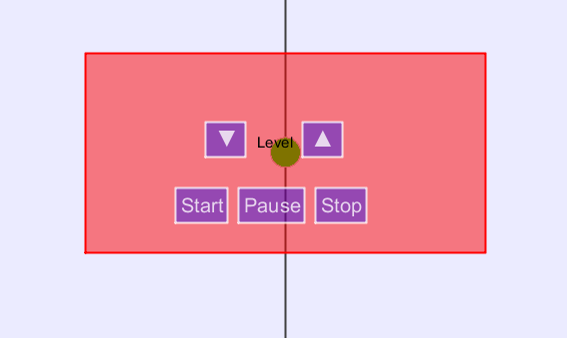
\includegraphics{../img/pong.png}
\end{center}

\end{multicols}

%%%LOCALIZE

\end{document}